\documentclass{beamer}

\usetheme[
    block=fill,
    background=light,
    titleformat=smallcaps,
    numbering=none
]{metropolis}

\usepackage{tabularx}
\usepackage{wasysym}
\usepackage{amsmath}
\usepackage{amssymb}
\usepackage{mathtools}
\usepackage{proof}
\usepackage{pifont}
\usepackage{algpseudocode}
\usepackage{algorithmicx}
\usepackage{tikz}
\usetikzlibrary{calc}
\usetikzlibrary{matrix}
\usetikzlibrary{positioning}
\usepackage{soul}
\usepackage{qtree}


\newcommand{\owl}{
\includegraphics[scale=0.04]{owl.png}}
\newcommand{\flamingo}{
\includegraphics[scale=0.02]{flamingo.pdf}}

\title{Typed Supertags and Semantic Parses for Dutch}
\institute{\owl UiL-OTS Utrecht University, \flamingo Universit{\'e} de Montpellier, CNRS}
\author{Konstantinos Kogkalidis\textsuperscript{\owl}, Michael Moortgat\textsuperscript{\owl}, Richard Moot\textsuperscript{\flamingo}}
\date{January 2020}

\algnewcommand\algorithmicforeach{\textbf{for each}}
\algdef{S}[FOR]{ForEach}[1]{\algorithmicforeach\ #1\ \algorithmicdo}


\begin{document}

\maketitle

\begin{frame}{Overview}
	\begin{itemize}
	\item[$\lambda$] {\textbf{Introduction}  {\footnotesize\textit{(or: why types?)}}\\
	 Type-Logical Grammars
	 }
	\item[$\lambda$] {\textbf{Framework} {\footnotesize\textit{(or: types, how?)}}\\
	Type System}
	\item[$\lambda$] {\textbf{Resources} \\
	Type Lexicon\\
	Semantic Parses
	}
	\item[$\lambda$] \textbf{Use Cases}
	\end{itemize}
\end{frame}

\begin{frame}{Type-Logical Grammars}

	\begin{block}{TL;DR}
		Words assigned \textit{formulas}, 
parsing a process of formal \textit{deduction}.
	\end{block}
	\vfill
	
	\textbf{Syntax}
	\begin{itemize}
	\item[] Structural Well-Formedness $\equiv$ Derivability
	\end{itemize}
	\vfill
	
 	\pause	
	\textbf{Curry-Howard Isomorphism}
	\begin{itemize}
	\item[] Propositions $\equiv$ Types
	\item[] Proofs $\equiv$ Functional Programs
	\end{itemize}
	\vfill
	
	\textbf{Syntax-Semantics Interface}
	\begin{itemize}
	\item[] Parse $\equiv$ Proof $\equiv$ Computational Terms
	\end{itemize}
\end{frame}

\begin{frame}{Type System (1/2)}
	\vfill
	\begin{block}{IILL}
	\centering
$
		\mathcal{T} := A \ | \ T_1 \multimap T_2 \
$
	\end{block}
	\vspace{-20pt}

	\begin{align*}
	A \in \mathcal{A} &{\quad::\quad} 
		\text{Atoms denoting complete phrases}\\
	{} & 	\text{
		\alert{
		\scriptsize
		N, NP, PRON, S \dots
		}
	}\\	
	T_1 \multimap T_2 &{\quad::\quad}
		\text{Linear functor from $T_1$ to $T_2$}\\
	{} & 
	\text{
		\alert{
		\scriptsize
		NP $\multimap$ S, NP $\multimap$ NP, NP $\multimap$ NP $\multimap$ S,
		(NP $\multimap$ NP) $\multimap$ (NP $\multimap$ NP)
		}
	}	
	\end{align*}

	\pause
	\begin{equation*}
	\infer[E]{\Gamma,\Delta\vdash (M\ N): {B}}{\Gamma\vdash M: A \multimap {B} & \Delta\vdash N: {A}}
	\end{equation*}
	\vfill
	\begin{equation*}
    \infer[I]{\Gamma \vdash \lambda x.M: {A}\multimap {B}}{\Gamma, x: {A} \vdash M: {B}}
	\end{equation*}
	\vfill
\end{frame}

\begin{frame}{Type System (2/2)}	
	\begin{block}{Modal Decoration Refinement}
	\centering
$
		\mathcal{T} := \color{gray}{A \ | \ T_1 \multimap T_2 \ } \color{black}{
		| \ \diamond^d {T_1} \multimap T_2 \ 
		| \ \Box^d ({T_1} \multimap T_2) }
$
	\end{block}
	\vspace{-20pt}
	
	\begin{align*}
	d \in \mathcal{D} &{\quad::\quad} 
		\text{Dependency relations}\\
	{} & 	\text{
		\alert{
		\scriptsize
		subj, dobj, body, mod, app, det \dots
		}
	}\\	
	\diamond^d T_1 \multimap T_2 &{\quad::\quad}
		\text{\footnotesize .. head fn selecting complement with dependency role $d$}\\
	{} & 
	\text{
		\alert{
		\scriptsize
		$\diamond^{subj}$ NP $\multimap$ S, $\diamond^{dobj}$ NP $\multimap$ $\diamond^{subj}$ NP $\multimap$ S, \dots
		}
	}\\	
	\Box^d (T_1 \multimap T_2)  &{\quad::\quad}
		\text{\footnotesize .. non-head fn projecting dependency $d$ }\\
	{} & 
	\text{
		\alert{
		\scriptsize
		$\Box^{det}$ (N $\multimap$ NP), $\Box^{mod}$ (NP $\multimap$  NP)
		}
	}	
	\end{align*}
\end{frame}

{
\setbeamercolor{background canvas}{bg=white}
\begin{frame}{Ducks, in Lassy}
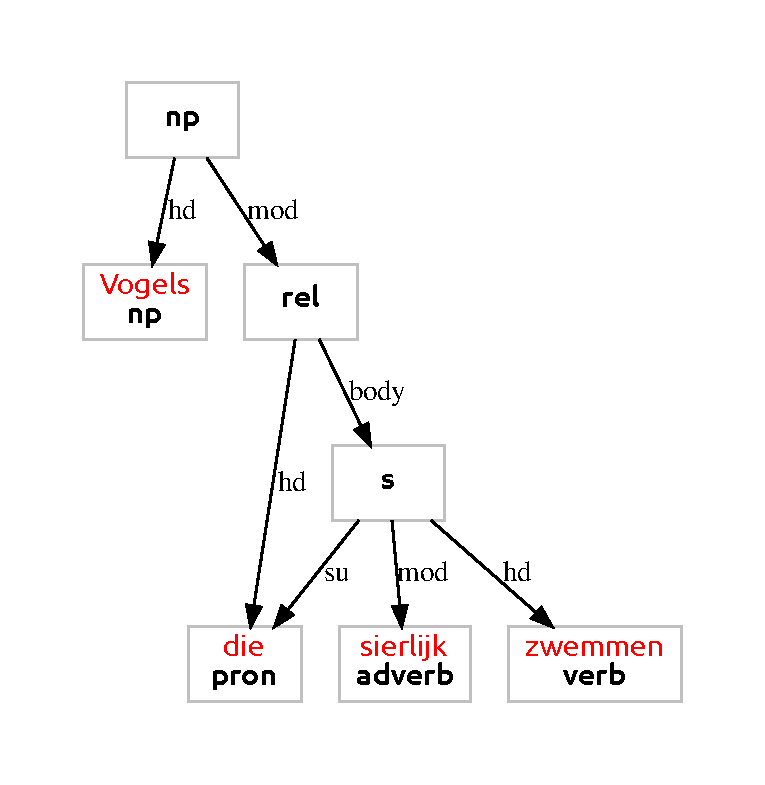
\includegraphics[width=\textwidth,height=\textheight,keepaspectratio]{quackers.pdf}\end{frame}
}

\begin{frame}{Ducks, Proven}
	\tiny

	\vfill
	\infer[E]{
		\textit{vogels}
		\left\langle 		
		\textit{die}
		\left\langle
		\left\langle \textit{sierlijk} \right\rangle^{mod}			\textit{zwemmen}
		\right\rangle^{body}		
		\right\rangle^{mod} \vdash 
		NP
		}{
		\infer[\mathcal{L}]{
			NP}{\text{\textit{vogels}}}
		&
		\infer[E]{
			\text{die} \left\langle \left\langle \text{sierlijk} \right\rangle^{mod} \text{zwemmen} \right\rangle^{body} \vdash
%			\text{die sierlijk zwemmen} \vdash
			\Box^{mod} (NP \multimap NP)}
			{
			\infer[\mathcal{L}]{
				RELPRO^{\color{red} 1}}{die}
%				\diamond^{body}(\diamond^{subj} NP \multimap S) \multimap \Box^{mod} (NP \multimap NP)}{die}
			&
			\infer[I]{
				\left\langle \text{sierlijk} \right\rangle^{mod} \text{zwemmen}
%				\text{sierlijk zwemmen} 
				\vdash 
				\diamond^{subj} PRON \multimap S}{
					\infer[E]{
						\left\langle PRON \right\rangle^{subj}
%						\diamond^{subj}PRON,\ 
						\left\langle \text{sierlijk} \right\rangle^{mod} \text{zwemmen}
%						\text{sierlijk zwemmen} 
						\vdash
						S
					}{
						\infer[E]{
							\langle PRON \rangle^{subj} 						
							%\diamond^{subj}PRON, 
							\text{zwemmen}
							 \vdash
							S}{
							\infer[Ax]{
							\diamond^{subj}PRON}{}
							&
							\hspace{2.5pt}
							\infer[\mathcal{L}]{\diamond^{subj}PRON \multimap S}{\text{\textit{zwemmen}}}
						}
						&
						\hspace{8pt}
						\infer[\mathcal{L}]{
							\Box^{mod} (S \multimap S)}{\text{\textit{sierlijk}}}
					}
				}
			}
		}
		\vfill
		
	\scriptsize
	
	
	\[
		\texttt{die}\left(\lambda x.\left(\texttt{sierlijk} \ \left(\texttt{zwemmen} \ x\right)\right)\right) \ \texttt{vogels}
	\]
	\vfill
	
	\begin{flushleft}
	{\color{red} 1}: $RELPRO := \diamond^{body} (\diamond^{su} PRON \multimap S) \multimap \Box^{mod} (NP \multimap NP)$
	\end{flushleft}
			
\end{frame}

\begin{frame}{\AE THEL}

	\begin{block}{Extraction}
	From Lassy Parses to IILL Types \& Theorems
	\begin{flushright}
	\textbf{arxiv}: \quad \texttt{abs/1912.12635}
	\end{flushright}
	\end{block}
	\vfill

	\textbf{Resources}	
	\begin{itemize}
	\item[\textbf{1}] Type Lexicon: Word $\to$ Type Distribution
	\item[\textbf{2}] Proofs: Lassy DAG $\to$ IILL Proof
	\begin{flushright}
		\footnotesize
			$\sim97\%$ \textit{coverage}
	\end{flushright}
	\end{itemize}
	
	\small{
	Wikipedia subset publicly available at
	\url{github.com/konstantinosKokos/aethel-public}}
		
\end{frame}

{
\setbeamercolor{background canvas}{bg=white}
\begin{frame}{\AE THEL: Lexicon}
	\textbf{Stats}
	\begin{itemize}
	\item $\sim$900\,000 word \& type pairs
	\item 81\,730 unique words
	\item 5\,771 unique semantic types
	\end{itemize}

	\begin{minipage}{0.725\textwidth}
	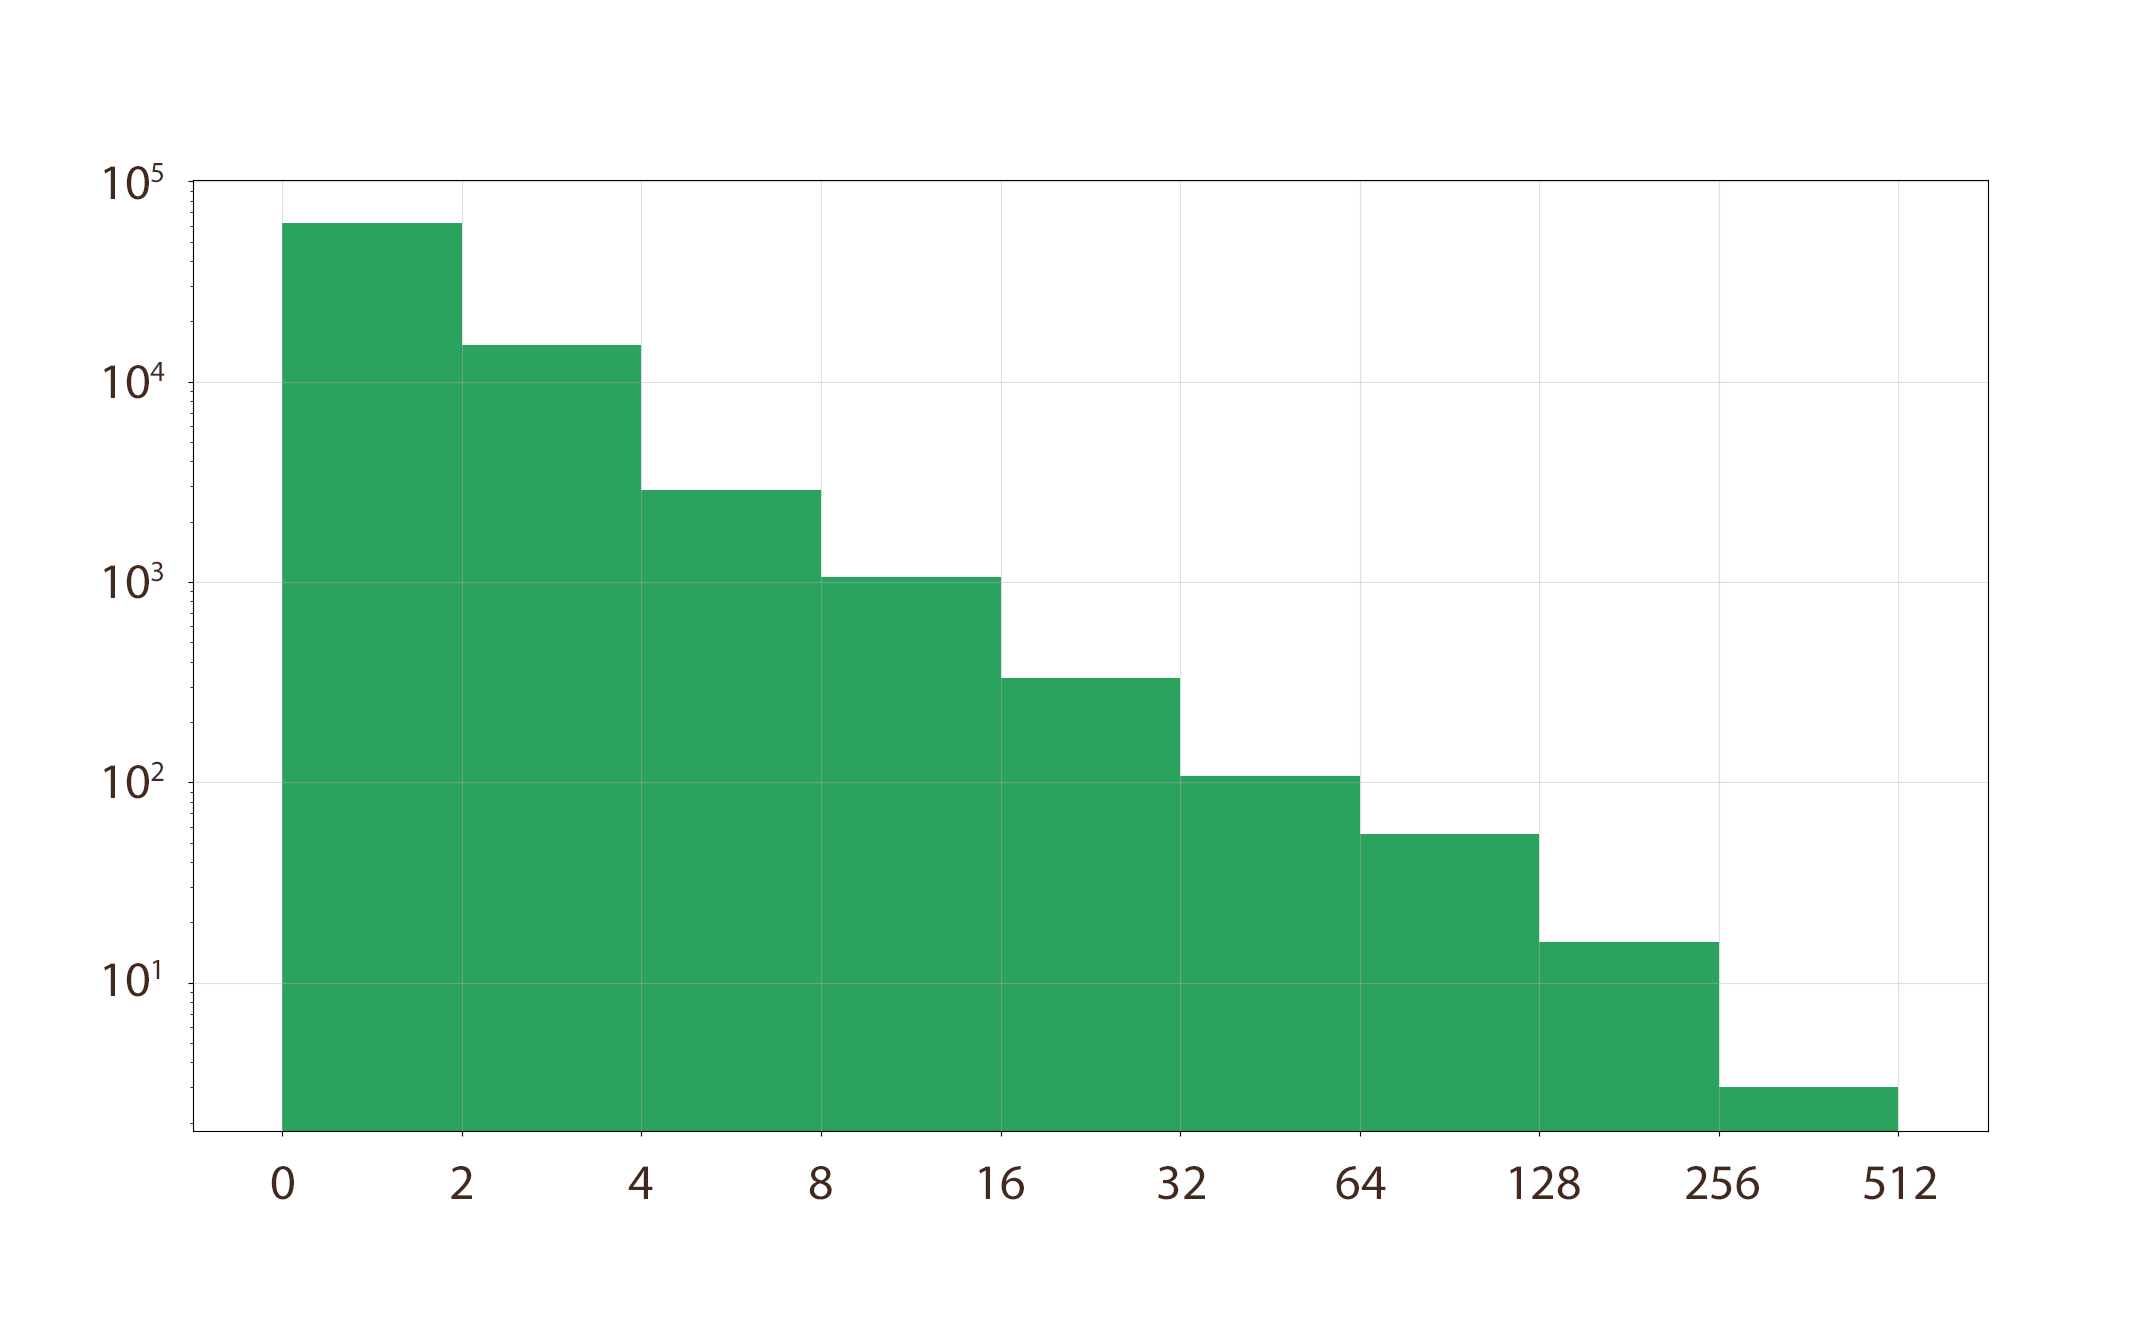
\includegraphics[width=\textwidth,height=0.65\textheight,keepaspectratio]{figure_2_2.png}	
	\end{minipage}%
	\begin{minipage}{0.275\textwidth}
	\scriptsize{Lexical Type Ambiguity Histogram\\
	(\textit{log10-log2})}
	\end{minipage}
\end{frame}


\begin{frame}{\AE THEL: Proofs}

	\begin{minipage}[t]{0.5\textwidth}
	\textbf{Formats}
	\begin{itemize}
	\item N.D. Proofs
	\item S.S. Proofs
	\item Linear Proofnets
	\item $\lambda$-terms
	\end{itemize}	
	\end{minipage}%
	\begin{minipage}[t]{0.5\textwidth}
	\textbf{Stats}
	\begin{itemize}
	\item 65\,020 Lassy DAGs
	\item 72\,263 IILL Proofs
	\end{itemize}
	\end{minipage}
	
	\begin{minipage}{0.75\textwidth}	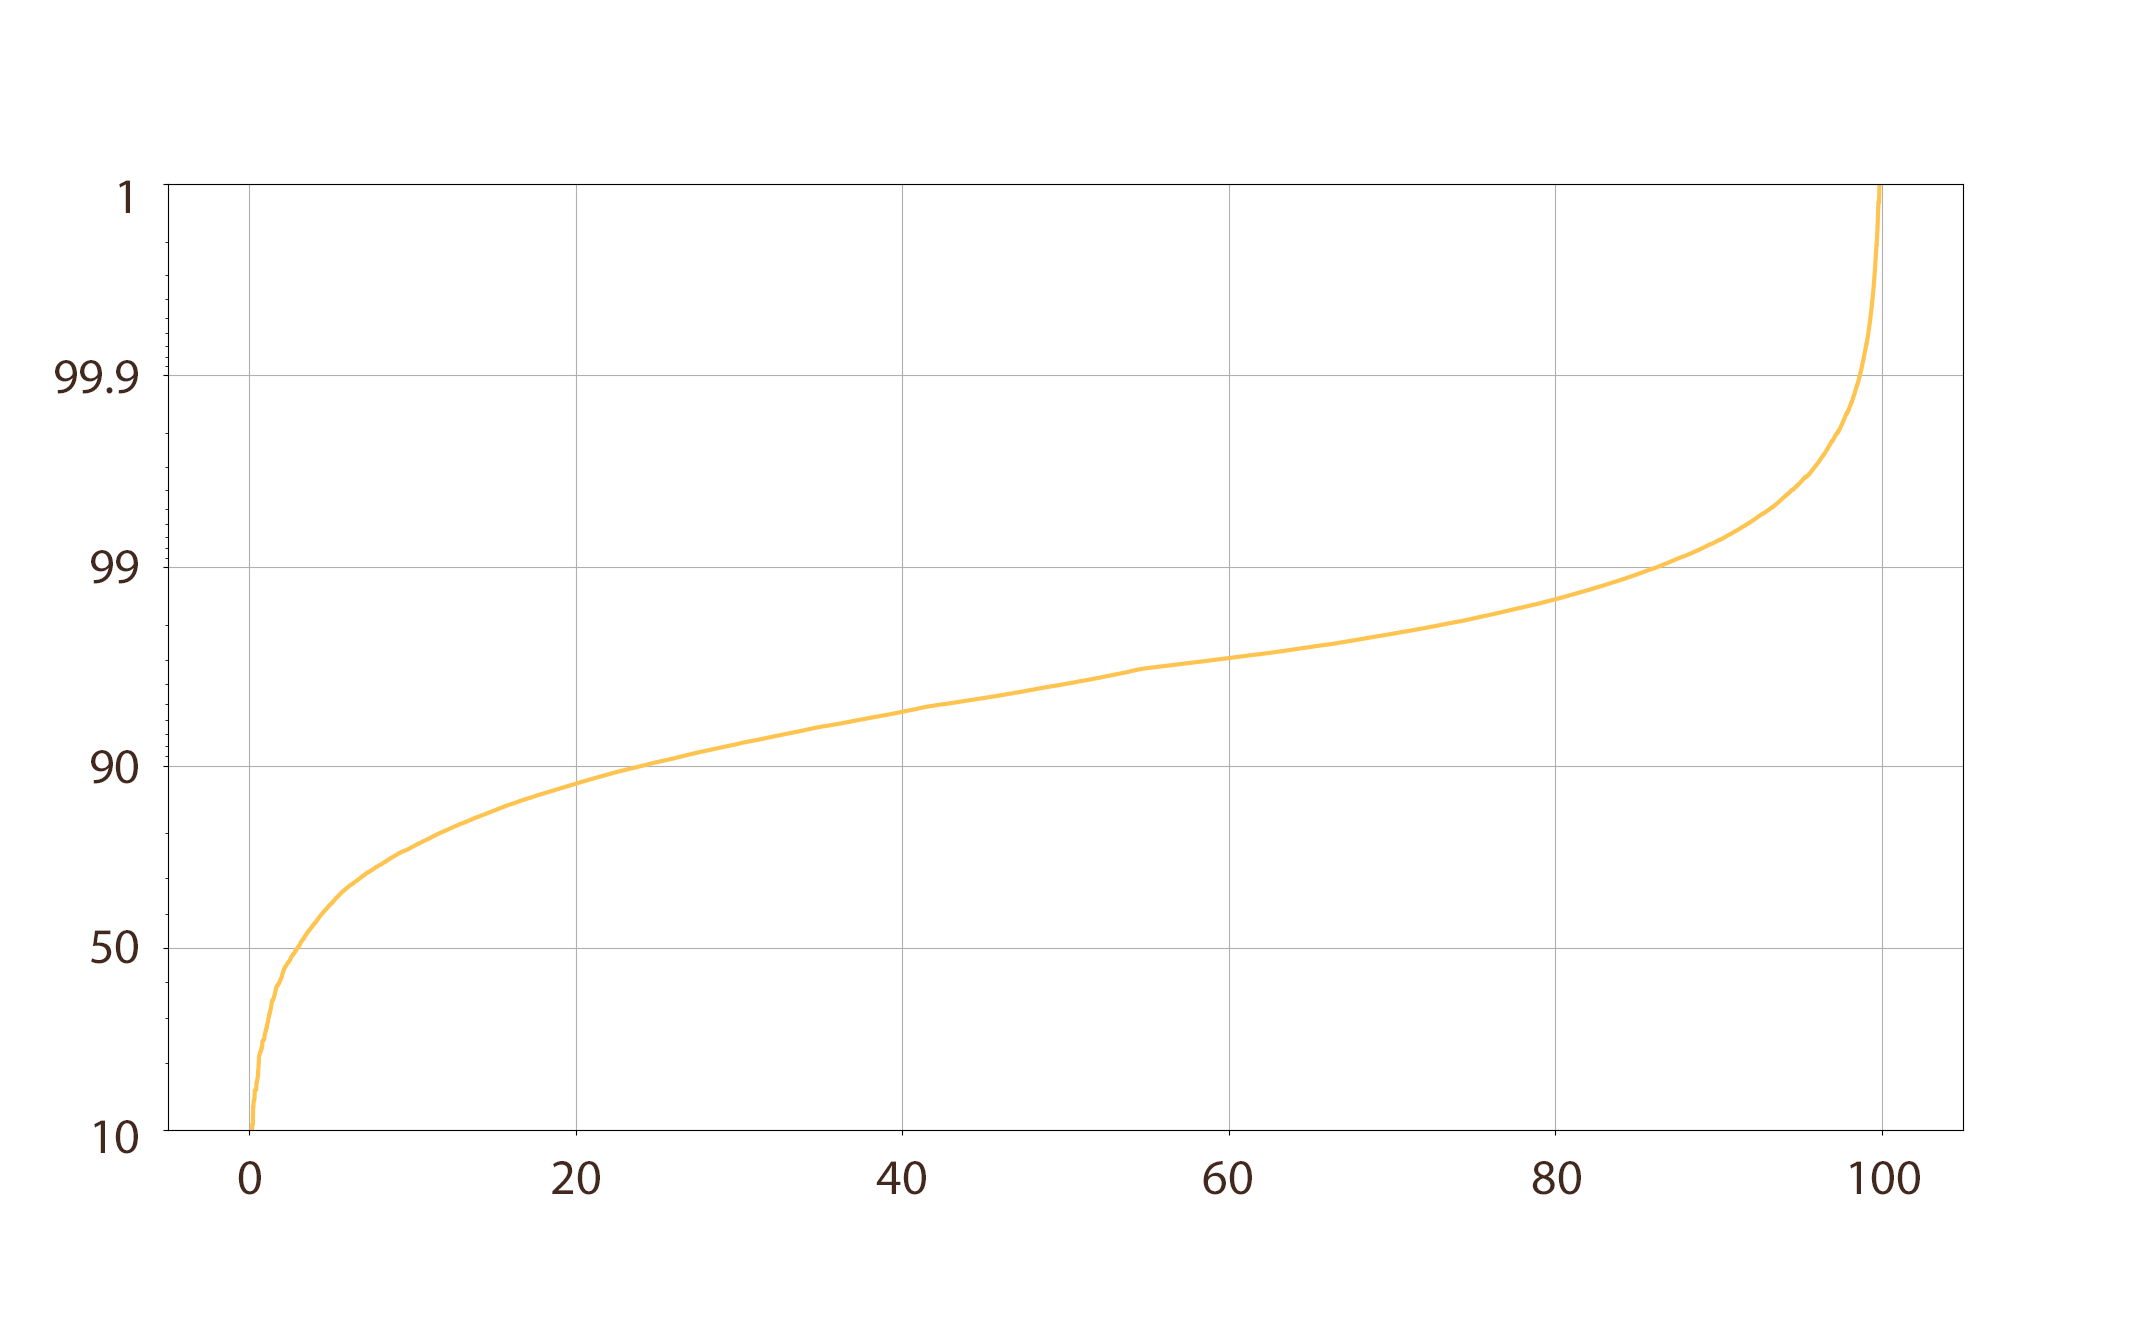
\includegraphics[width=\textwidth,height=0.6\textheight,keepaspectratio]{sentence_covr3.png}\end{minipage}%
	\begin{minipage}{0.25\textwidth}
	\scriptsize{Proof coverage w.r.t. most frequent types\\
	(\textit{logit-linear})}
	\end{minipage}
	
\end{frame}
}

\begin{frame}{Use Cases \& Applications}
	\begin{itemize}
	\item {Supertagging with no type lexicon\\
	\begin{flushright}
	\textbf{arxiv}: \quad \texttt{abs/1905.13418}	
	\end{flushright}
	}
	\item {Parsing with type hints
	\begin{flushright}
	\textbf{hal-lirmm}: \quad \texttt{lirmm-02313572}	
	\end{flushright}
	}
	\item {Type-aware language modeling}
	\item {Text to $\lambda$-term translation}
	\item {Semantic Compositionality}
	\item {...?}
	\end{itemize}
	
\end{frame}

%\begin{frame}{Why Types?}
%	\begin{minipage}[t]{0.65\textwidth}
%	\invisible<1>{
%	\textbf{Type-Logical Grammars}
%	\begin{itemize}
%		\item[] Words $\rightarrow$ Logical Formulas
%		\item[] Well-Formedness $\equiv$ Provability
%	\end{itemize}}
%	\vfill	
%		
%	\visible<3->{
%	\textbf{Curry-Howard Correspondence}
%	\begin{itemize}
%		\item[] Logical Formulas $\leftrightarrow$ Typed Variables
%		\item[] Proofs $\equiv$ Functional Programs
%	\end{itemize}}
%	
%	\visible<4->{\textbf{Syntax-Semantics Interface}
%	\begin{itemize}
%		\item[] Syntactic Types $\to$ Semantic Spaces
%		\item[] Derivations $\to$ Semantic Programs
%	\end{itemize}
%	}
%\end{minipage}%
%	\begin{minipage}[t]{0.35\textwidth}
%		\begin{figure}
%	\begin{tikzpicture}[
%		dot/.style={circle, inner sep=0pt, outer sep=4pt, minimum size=0pt, fill=black}
%	]
%		\visible<2->{\node[dot, label=right :{\small Logic}] (lo) at (0, 0) {};}
%		\visible<1->{\node[dot, label=left:{\small Syntax}] (la) at ($(lo)+(0:-2)$) {};}
%		\visible<3->{\node[dot, label={[yshift=-20pt]\small Computation}] (co) at ($(la)+(-60:2)$) {};}
%		\visible<4->{\node[dot, label={[yshift=-20pt]\small Semantics}] (sem) at ($(co) + (0,-2)$) {};}		
%				
%		\visible<2->{\draw (lo) edge[<->, thick] node[midway, above] {\footnotesize TLG} (la);}
%		\visible<3->{\draw (la) edge[<->, thick] (co);}
%		\visible<3->{\draw (co) edge[<->,  thick] node[midway, right] {\footnotesize CHC} (lo);}
%		
%		\tikzset{decoration={snake,amplitude=.4mm,segment length=2mm,
%                       post length=0mm,pre length=0mm}}
%         \visible<4->{\draw [->, line join=round, decorate, decoration={	zigzag, segment length=4, amplitude=.9, post=lineto, post length=2pt}] ($(co.south) + (0, -.35)$) -> (sem);
%		\node[label=above:{\footnotesize hom}] at (-0.5,-3.25) {};}
%	\end{tikzpicture}
%\end{figure}	
%	\end{minipage}
%\end{frame}


%\begin{frame}{Overview}
%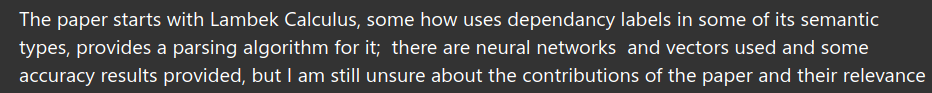
\includegraphics[keepaspectratio,width=\textwidth]{intro.png}\vfill
%
%\pause
%\begin{itemize}
%	\item[$\lambda$] Abstract Syntax with NLP
%	\item[$\lambda$] Extracting \& Learning Type Assignments
%	\item[$\lambda$] Navigating proofs with neural nets
%	\item[$\lambda$] Lexicalized syntax in language modeling
%\end{itemize}
%
%\end{frame}
%
%\begin{frame}{This Timeline}
%	\begin{tikzpicture}
%		\node (syntax) at (0,0) {\scriptsize Syntactic Derivations};	
%		\node (nl) at (0,0.7) {\scriptsize (N)L};
%		\node (der) at (4,0) {\scriptsize Derivational Semantics};
%		\node (mill) at (4,0.7) {\scriptsize LP};
%		\node (sem) at (8,0) {\scriptsize Lexical Semantics};
%		\node (il) at (8, 0.7) {\scriptsize IL};
%
%		\draw (syntax) edge[->] node[midway, above] {\footnotesize $h_{der}$} (der);
%		\draw (der) edge[->] node[midway, above] {\footnotesize $h_{lex}$} (sem);
%	\end{tikzpicture}	
%\end{frame}
%
%\begin{frame}{Alternative Timeline}
%	\begin{tikzpicture}
%		\visible<2->{
%			\node (syntax) at (0,0) {\scriptsize \color{gray}{Syntactic Derivations}};
%			\node (nl) at (0, 0.5) {\scriptsize \color{gray}{?}};}			
%%		\node (abstract) at (2, 2) {\scriptsize wtf};		
%		\node (der) at (4,1.5) {\scriptsize \color{red}{Abstract Syntax}};
%		\node (nlp) at (4, 2.2) {\scriptsize \color{red}{NLP}};
%		\node (sem) at (8,0) {\scriptsize Lexical Semantics};
%		\node (il) at (8, 0.7) {\scriptsize IL};
%		
%		\visible<2->{\draw (der) edge[->, gray] node[midway, above] {\footnotesize \color{gray}{?}} (syntax);}
%		\draw (der) edge[->] node[midway, above] {\footnotesize $h_{lex}$} (sem);		
%	\end{tikzpicture}
%\end{frame}
%
%\begin{frame}{NLP}
%
%	\begin{block}{Grammar}
%		IILL + Structural Control Modalities
%	\end{block}
%	\vfill	
%	
%	\[
%		\mathcal{T} := A \ | \ \diamond^d{T}_1 \to T_2 \
%	\]
%	\vfill 
%	
%	\begin{align*}
%		A \in \mathcal{A} &{\quad::\quad} 
%			\text{Atoms denoting complete phrases \scriptsize {(NP, S, \dots)}}\\
%		d \in \mathcal{D} &{\quad::\quad}  
%			\text{Grammatical relations \scriptsize{(subject, object, \dots)}} \\
%		\diamond^dT &{\quad::\quad} 
%			\text{Type demarkated by \textit{dependency domain} d}\\
%		T_1 \to T_2 &{\quad::\quad} 
%			\text{Linear functor from $T_1$ to $T_2$}
%	\end{align*}
%\end{frame}
%
%
%\begin{frame}{	
\includegraphics[keepaspectratio,width=\textwidth]{but_why.png}	}
%	
%	\textbf{Why?}
%	\begin{itemize}
%		\item Easier to extract from corpora
%		\item Drastic reduction in lexical ambiguity
%		\item More informative for semantics
%		\item Built-in Interpretability
%		\item Diamonds can regulate parsing (?)
%	\end{itemize}\vfill	
%	
%	\pause
%	\textbf{How?}
%	\small
%		\begin{equation*}
%			\infer[\to  E]{\Gamma,\Delta\vdash (M\ N): {B}}{\Gamma\vdash M: A \to {B} & \Delta\vdash N: {A}}
%		\end{equation*}
%		\begin{equation*}
%		    \infer[\to I]{\Gamma \vdash \lambda x.M: {A}\to {B}}{\Gamma, x: {A} \vdash M: {B}}
%		\end{equation*}
%		\begin{equation*}
%		    \infer[\diamond^d I]{\langle \Gamma \rangle^d \vdash \diamond^d {A}}{\Gamma \vdash {A}}
%		\end{equation*}
%		\begin{equation*}
%			\infer[\diamond^d E]{\Gamma,\Delta \vdash {B}}{\Delta \vdash \diamond^d {A}
%			&
%			\Gamma,\langle {A} \rangle^d \vdash {B}}
%		\end{equation*}	
%\end{frame}
%
%\begin{frame}{}
%	\centering
%	\alert{
%		A dataset of types \& proofs
%	}
%\end{frame}
%
%\begin{frame}{Extracting (1/3)}
%\small
%
%	\begin{block}{Algorithm}
%		Graph flooding on syntactic parse graphs \\
%		Init with maps:
%		\begin{itemize}
%			\item[-] from POS/Phrasal-tags to atoms
%			\item[-] dependency labels to diamond operators
%		\end{itemize}
%		Two subroutines;
%			each \textit{selects} untyped nodes and \textit{types} them
%	\end{block}
%	
%	\pause	
%	\vfill
%	\begin{algorithmic}
%	\Function{TypeDag: DAG $D$ $\to$ DAG}{}
%		\State $D$ $\gets$ DetachNonLocal($D$)
%		\While{$D$ is not fully typed}
%			\State $D$ $\gets$ TypeStandaloneNodes($D$)
%			\State $D$ $\gets$ TypeHeadsAndMods($D$)
%		\EndWhile\\
%		\Return AttachNonLocal($D$)
%	\EndFunction
%	\end{algorithmic}
%\end{frame}
%
%\begin{frame}{Extracting (2/3)}
%\small
%
%	\begin{itemize}
%		\item[$\lambda$1] Stand-Alone Nodes
%			\begin{itemize}
%				\setlength{\itemindent}{.25in}
%				\item[select] untyped nodes with
%					\begin{itemize}
%						\item[1] no incoming head/mod edge
%						\item[2] no untyped daughters (except heads/mods)
%					\end{itemize}
%				\item[type] translate pos/tag to atom
%			\end{itemize}\vfill
%		\item[$\lambda$2] Heads and Mods
%			\begin{itemize}
%				\setlength{\itemindent}{.25in}
%				\item[select] untyped nodes that
%					\begin{itemize}
%						\item[1] incoming head/mod edge
%						\item[2] have a typed parent
%						\item[3] have all sisters (except head/mods) typed
%					\end{itemize}
%				\item[type] endofunctor of parent if mod, else functor from vector of arguments\footnote{minus hypotheses} to parent type
%			\end{itemize}
%	\end{itemize}
%
%\end{frame}
%
%
%\begin{frame}{Extracting (3/3)}
%
%	\begin{block}{Non-Local Dependencies}
%	\begin{algorithmic}
%	\Function{DetachNonLocal: DAG $D$ $\to$ Tree}{}
%		\ForEach {$e$ $\in$ $\textsc{Filter(Reentrant}, D.edges)$}
%			\State $c$ $\gets$ copy$(e.target)$
%			\State $D.nodes$ $\gets$ $D.nodes \cup \{c\}$
%			\State $D.edges$ $\gets$ $D.edges - \{e\}$
%			\State $D.edges$ $\gets$ $D.edges \cup \{(e.source, e.label, c)\}$
%		\EndFor\\
%		\Return $D$
%	\EndFunction
%	\end{algorithmic}
%	\end{block}	
%\end{frame}
%
%\begin{frame}{}
%	\centering
%		\alert{Mommy, where do types come from?}
%
%\end{frame}
%
%\begin{frame}{Lexical Type Ambiguity}
%
%	\begin{block}{Word/Type histogram}
%	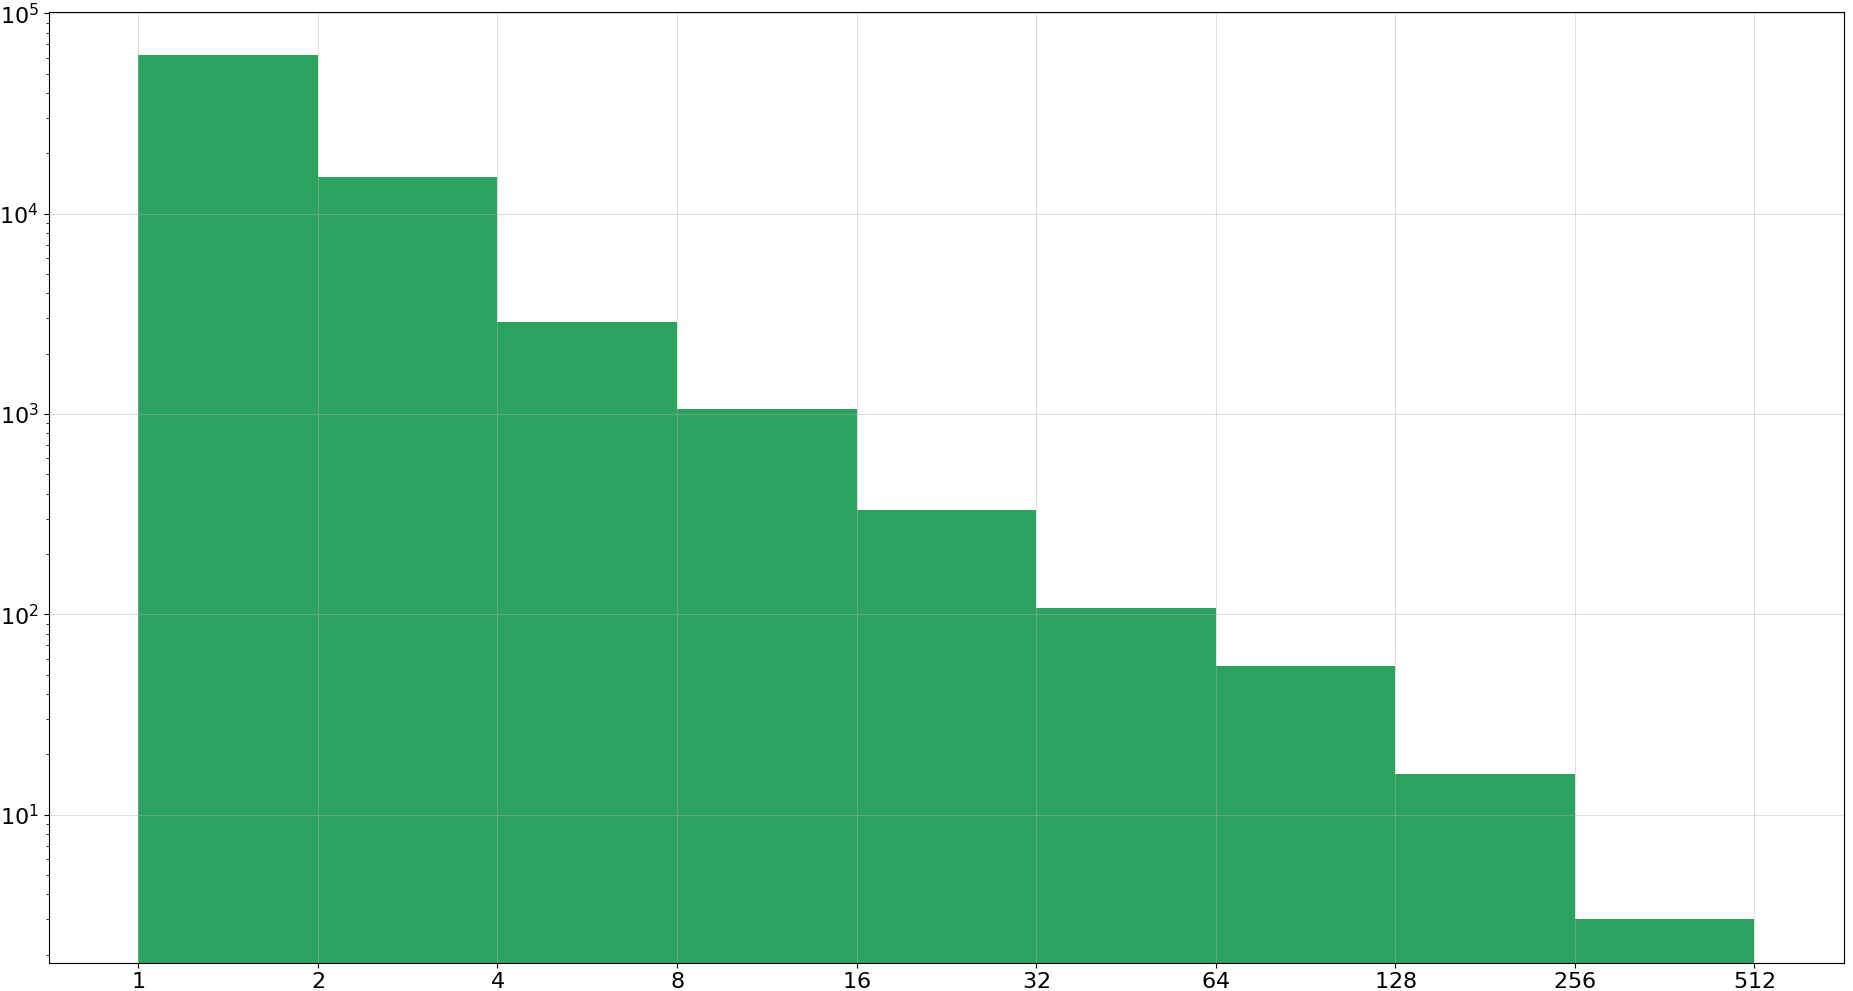
\includegraphics[keepaspectratio,width=\textwidth]{oracle.png}
%	\end{block}
%\end{frame}
%
%\begin{frame}{Supertagging (\alt<3->{2}{1}/3)}
%	\small	
%	
%	\begin{block}{General idea}
%		\[
%			p(t_1, t_2, \dots t_n | w_1, w_2, \dots w_n, \theta)
%		\]
%	\end{block}\vfill
%	
%	\begin{block}{\alt<3->{\st{Markov Assumption}}{Markov Assumption}}
%		\alt<3->{
%		\[
%			\approx \prod_{i=1}^n p(t_i | t_1, \dots t_{i-1}, w1, \dots, w_n, \theta)
%		\]
%		}{
%		\[
%			\approx \prod_{i=1}^n p(t_i | w_1, w_2, \dots w_n, \theta)
%		\]
%		}
%	\end{block}\vfill
%
%	\begin{itemize}
%		\item[\smiley] Seq2Seq \alt<3->{\alert{Transduction}}{Classification}
%		\item[\alt<3->{\smiley}{\frownie}] \alt<3->{\alert{Many Answers}}{Single Answer}
%		\item[\frownie] Sample Sparsity
%		\item[\frownie] Closed Domain Assumption 
%	\end{itemize}
%\end{frame}
%
%\begin{frame}{Supertagging (3/3)}
%	\small
%	\begin{block}{A step further}
%		The syntax of the type system forms a simple CFG
%		\begin{align*}
%			S & \implies A \  &\forall \ A \ \in \ \mathcal{A}\\
%			S & \implies d \ S \ S \ &\forall \ d \ \in \ \mathcal{D}
%		\end{align*}
%	\end{block}
%	
%	\pause
%	\begin{itemize}
%		\item Supertagging as conditional CFG generation
%		\item CFG terminals as decoding targets
%			\[
%			\approx \prod_{i=1}^{\alert{m}} p(\alert{\sigma_i} | \alert{\sigma_1}, \dots \alert{\sigma_{i-1}}, w1, \dots, w_n, \theta)
%			\]
%			\[
%				\sigma \in \mathcal{A} \cup \mathcal{D} \cup \{ \textsc{\scriptsize <SEP>} \}
%			\]
%	\end{itemize}
%	
%	\pause
%	\begin{itemize}
%		\item[\smiley] \st{Sample Sparsity} Many (sub)type examples
%		\item[\smiley] \st{Closed Domain Assumption} Inductive construction of any type
%	\end{itemize}
%	
%\end{frame}
%
%\begin{frame}{}
%	\centering
%	\alert{
%		Structural Ambiguity
%	}
%\end{frame}
%
%\begin{frame}{Navigating Proofs}	
%
%	\begin{block}{Parse State}
%		\begin{itemize}
%			\item A logical judgement (premises \& conclusion)
%			\item Word associations for (some) premise formulas
%			\item A single element stack
%		\end{itemize}
%	\end{block}
%	
%	\pause
%	\begin{block}{Framework}	
%		Given a parse state:
%		\begin{itemize}
%			\item[1] Decide between introduction $\oplus$ elimination
%			\item[2] Perform either
%			\item[3] Update state(s) 
%			\item[4] Repeat
%		\end{itemize}		
%	\end{block}
%\end{frame}
%
%\begin{frame}{Proof Ambiguity}
%
%	\begin{block}{The Problem}
%		\begin{itemize}
%			\item Introduction steps are deterministic
%			\item Eliminations are not
%		\end{itemize}
%	\end{block}\vfill
%	
%	\pause
%	\begin{block}{Key Insight}
%		Elimination branching $\sim$ binary sequence chunking\\
%		Semantic content can help disambiguate structure\\
%	\end{block}\vfill
%	
%\end{frame}
%
%\begin{frame}{Vectorizing Types}	
%	\small
%	
%	\begin{block}{Types are trees}
%	\centering 
%	\[
%		\diamond^{body}(\diamond^{su} NP \to S) \to \diamond^{mod} NP \to NP
%	\]
%	\end{block}
%
%	\centering
%	{\scriptsize
%	\begin{minipage}{0.5\textwidth}
%		\Tree[.{$\to$}	[.{$\diamond \ body$} [.{$\to$} [.{$\diamond \ {su}$} NP ] S ] ] [.{$\to$} [.{$\diamond \ mod$} NP ] NP ] ] 
%	\end{minipage}
%	}\vfill
%	
%	\pause
%	\centering
%	\begin{itemize}
%		\item Atoms as vectors in $\mathbb{R}^n$
%		\item Dependencies as functions $\mathbb{R}^n \to \mathbb{R}^n \to \mathbb{R}^n$
%	\end{itemize}
%\end{frame}
%
%\begin{frame}{Proof Traversal}
%
%    {
%    \scriptsize
%    \begin{minipage}{0.3\textheight}
%    	\infer[]{\text{ducks}, \text{have}, \text{many}, \text{predators} \vdash \text{S}}{
%	    	\infer[Ax.]{\text{\color<2>{red} ducks} \vdash \text{NP}}{}
%	    	&
%	    	\hspace{-20pt}
%    		\infer[\rightarrow E]{\text{have}, \text{many}, \text{predators} \vdash \text{NP} \to \text{S}}{
%    			\infer[\rightarrow E]{\text{\color<4>{red}many}, \text{\color<4>{red}predators} \vdash \text{NP}}{
%    				\infer[Ax.]{\text{\color<6>{red} predators} \vdash \text{NP}}{}
%    				&
%    				\infer[Ax.]{\text{many} \vdash \text{NP} \to \text{NP}}{}
%    			}
%    			&
%    			\infer[Ax.]{\text{have} \vdash \text{NP} \to \text{NP} \to \text{S}}{}
%    		}
%    	} 
%    \end{minipage}
%    }\vfill
%    
%    \begin{minipage}{0.6\textheight}
%    \begin{figure}
%    \centering
%    \begin{tikzpicture}
%        \scriptsize
%        
%    	\node[rectangle, inner sep=0pt, minimum width=120pt, minimum height=20pt] (ducks) at (0, -1.5) {
%    		\alt<3->{
%    			\alt<5->{
%    				\alt<7->{
%    					\alt<9->{}
%    						{}}
%    				{many, {\color<6->{red}predators}}}
%    			{have, {\color<4->{red}many, predators}}}
%    		{{\color<2->{red}ducks}, have, many, predators}
%			\alt<7->{}{$\vdash$}
%			\alt<3->{
%				\alt<5->{
%					\alt<7->{}
%					{NP}}
%				{NP $\to$ S}}
%			{S}
%		};
%    	
%
%   	\node[draw=white, rectangle, minimum width=240pt, minimum height=20pt, ultra thick, fill=black] (bb) at (0, 0) {\color{white}{Sequence Processing Black Box}};
%   	
%    	\pause
%    	\node[rectangle, inner sep=0pt, minimum width=120pt, minimum height=20pt] (ducks) at (0, -1.5) {};
%    	\invisible<7->{\draw ($(ducks.north) + (0, 0)$) edge[->, ultra thick] node[above] {} ($(bb.south) + (0, 0)$);}
%    	
%		\node[rectangle, inner sep=0pt, minimum width=120pt, minimum height=20pt] (fst) at (-2.25, 1.25) {
%		{\alt<3->{}{{\color{red} L}}}};
%		
%		\node[rectangle, inner sep=0pt, minimum width=120pt, minimum height=20pt] (snd) at (-1.25, 1.25) {
%		{\alt<3->{
%			\alt<4->{
%				\alt<5->{
%					\alt<6->{\invisible<7->{R}}{}}{R}}{}
%%					\alt<6->{}{}}{R}}{}
%		}{R}}};
%		
%		\node[rectangle, inner sep=0pt, minimum width=120pt, minimum height=20pt] (trd) at (-0.25, 1.25) {
%		{\alt<3->{
%			\alt<4->{
%				\alt<5->{
%%					\alt<6->{\invisible<7->{R}}{}}{\color{red} L}}{}
%					\alt<6->{\invisible<7->{\color{red} L}}{}}{\color{red} L}}{}
%
%		}{R}}};
%		
%		\node[rectangle, inner sep=0pt, minimum width=120pt, minimum height=20pt] (fth) at (0.75, 1.25) {
%		{\alt<3->{
%			\alt<4->{
%				\alt<5->{
%					\alt<6->{}{}}{\color{red} L}}{}
%		}{R}}};
%		
%		\invisible<3->{
%			\draw ($(bb) + (-2.25, 0.25)$) edge[->, thick, red] node[above] {} ($(fst.south)$);
%			\draw ($(bb) + (-1.25, 0.25)$) edge[->, thick] node[above] {} ($(snd.south)$);
%			\draw ($(bb) + (-0.25, 0.25)$) edge[->, thick] node[above] {} ($(trd.south)$);
%			\draw ($(bb) + (0.75, 0.25)$) edge[->, thick] node[above] {} ($(fth.south)$);
%		}
%		
%	\alt<4->{
%	\invisible<5->{
%			\draw ($(bb) + (-1.25, 0.25)$) edge[->, thick] node[above] {} ($(snd.south)$);
%			\draw ($(bb) + (-0.25, 0.25)$) edge[->, thick, red] node[above] {} ($(trd.south)$);
%			\draw ($(bb) + (0.75, 0.25)$) edge[->, thick, red] node[above] {} ($(fth.south)$);
%		}
%	}{}
%	
%	\alt<6->{
%	\invisible<7->{
%			\draw ($(bb) + (-1.25, 0.25)$) edge[->, thick] node[above] {} ($(snd.south)$);
%			\draw ($(bb) + (-0.25, 0.25)$) edge[->, thick, red] node[above] {} ($(trd.south)$);
%		}
%	}{}
%    \end{tikzpicture}
%    \end{figure}
%    \end{minipage} 
%    \vfill 
%   
%	\only<8>{
%	\[
%	\begin{rcases*}
%		\text{Training sample} \ &: \ \text{Elimination branching} \\
%		\text{Sentence} \ 	&: \ \text{N \textit{independent} samples} \\
%	\end{rcases*}  \text{\alert{Training Parallelism}}
%	\]
%    }
%\end{frame}
%
%\begin{frame}{}
%	\centering
%	\alert{
%		Parsing in $\mathcal{O}$(1)
%	}\footnote{
%	\scriptsize Sensationalist}
%\end{frame}
%
%
%\begin{frame}{Parsing as Latent Permutation}
%	\[
%		\alt<2->{\alt<3->{np_1^+}{np_1}}{np}, 
%		\alt<2->{\alt<3->{np_2^-}{np_2}}{np} 
%		\to 
%		\alt<2->{\alt<3->{np_3^-}{np_3}}{np} 
%		\to 
%		\alt<2->{\alt<3->{s_1^+}{s_1}}{s}, 
%		\alt<2->{\alt<3->{np_4^-}{np_4}}{np} 
%		\to \alt<2->{\alt<3->{np_5^+}{np_5}}{np}, 
%		\alt<2->{\alt<3->{np_6^+}{np_6}}{np} 
%		\vdash 
%		\alt<2->{\alt<3->{s_2^-}{s_2}}{s}
%	\]\vfill
%
%	\pause
%	\pause
%	\pause
%	
%	\[
%		P = [np_1, s_1, np_5, np_6] \quad 		N = [np_2, np_3, np_4, s_2]
%	\]\vfill
%
%	\pause	
%	
%	\centering
%	\alt<6->{$\mathcal{R} \in \mathbb{B}^{4 \times 4}$ =}{} \begin{tabular}{c|cccc}
%		& $np_2$ & $np_3$ & $np_4$ & $s_2$\\
%		\hline
%		$np_1$ & \visible<6-> 0 & \alt<6->{1}{X} & \visible<6-> 0 & \visible<6-> 0 \\
%		$s_1$ &  \visible<6-> 0 &  \visible<6-> 0 &  \visible<6-> 0 & \alt<6->{1}{X} \\
%		$np_5$ & \alt<6->{1}{X} & \visible<6-> 0 & \visible<6-> 0 &  \visible<6-> 0\\
%		$np_6$ & \visible<6-> 0 & \visible<6-> 0 & \alt<6->{1}{X} &  \visible<6-> 0\\
%	\end{tabular} 
%	
%	\pause
%	\[
%		\text{match}(N) = P\mathcal{R}^T
%	\]
%	
%	\pause
%	\begin{itemize}
%		\item $\mathcal{R}$ is \textit{discrete}
%		\pause
%		\item .. but its continuous relaxations can be approximated (Sinkhorn-Knopp)
%	\end{itemize}	
%\end{frame}
%
%
%\begin{frame}{References}
%	\small 
%	
%	\begin{block}{Grammar \& Extraction}
%		\begin{itemize}
%			\item \AE THEL: Automatically Extracted Type-Logical Derivations for Dutch \href{https://arxiv.org/abs/1912.12635}{\color{blue}{link}}
%		\end{itemize}
%		
%	\end{block}
%	
%	\begin{block}{Supertagging \& Parsing}
%		\begin{itemize}
%			\item Constructive Type-Logical Supertagging with Self-Attention Networks \href{https://arxiv.org/abs/1905.13418}{\color{blue}link}
%			\item Deductive Parsing with an Unbounded Type Lexicon \href{https://hal-lirmm.ccsd.cnrs.fr/lirmm-02313572/document}{\color{blue}link}
%		\end{itemize}
%	\end{block}
%	
%	\begin{block}{Permutations}
%		\begin{itemize}
%		\item Sinkhorn-Knopp Algorithm \href{http://yaroslavvb.com/papers/sinkhorn-concerning.pdf}{\color{blue}link}
%		\item Learning Latent Permutations with Gumbel-Sinkhorn Networks \href{https://arxiv.org/abs/1802.08665}{\color{blue}link}
%		\end{itemize}
%	\end{block}
%\end{frame}

\end{document}